\subsection{Intrinsic roll over temperature}
\label{sec:eval:trollover}

One method to estimate the thermal resistance
looks at the dissipated power at roll over,
linked with the heat sink temperature --
see section~\ref{sec:rth:trollover}.
This method relies on an intrinsic roll over temperature,
independent of the heat sink temperature:
we associate
the longest emitted wavelength
with a temperature
in the active region.
If roll over occurs
because the active
exceeds a critical temperature,
the emitted wavelength
at this point
should be the same
regardless of the heat sink temperature
\begin{equation}
T_\mathrm{ro} = \Ths + \Rth D_\mathrm{ro}.
\end{equation}

We don't know
whether all VECSEL structures
show this behavior,
or whether it depends on the device.
It is thus necessary
to first test the hypothesis
by looking at the spectrum
emitted at roll over.
Once this is established
the method described
in section~\ref{sec:rth:trollover}
is more convenient
for estimating $\Rth$.

Our measurements
were pump limited.
Not every investigated 
spot size and heat sink temperature
did reach roll over.
This would be necessary
in order to extract
the thermal resistance
with said method.
However,
I can highlight
the emitted spectra
of those settings that did reach roll over.

The pump spot size scaling measurements
of sample 1
depicted in Fig.~\ref{img:Rth_lambda_spot_scaling}
suggest an ultimately
longest emitted wavelength
of about $1271\,\mathrm{nm}$.
In the case of the $180\,\mu\mathrm{m}$
the measurements corresponding to
a heat sink temperature of
\degr{30} and \degr{45}
both even out at this wavelength.

In the configuration
with lens $\mathrm{L}_\mathrm{p1}$
being achromatic
the observed spectrum behaves differently.
Figure~\ref{img:lambda_sample}
shows this exemplary
for the spectra
corresponding to
the measurements presented
in Fig.~\ref{img:LL_sample}.
The longest emitted wavelength
does not depend linearly
on dissipated power.

Consequentially,
I cannot apply the linear regression
suggested in \ref{sec:rth:lambda},
\cite{Heinen2012},
in order to extract $\Rth$.
In principle,
I could evaluate the derivatives
$\frac{\partial \lambda}{\partial D}$
and $\frac{\partial \lambda}{\partial T}$
numerically.
However,
due to the fluctuations on $D$
it is not clear
how to evaluate
$\frac{\partial \lambda}{\partial T}$
in practice.
I therefore withstand
to call out a number for $\Rth$
based on the presented results.

Concerning longest emitted wavelength,
in Fig.~\ref{img:lambda_sample}
we see the measurements
corresponding to
$\Ths=\{48,38,29\}\,^\circ\mathrm{C}$
to converge to the same value.
This limit wavelength is,
however,
longer than suggested
by Fig.~\ref{img:Rth_lambda_spot_scaling}.
The spectrum of sample 2,
plotted in Fig.~\ref{img:lambda_sampled6},
does not allow to infer
on the behavior of the peak wavelength.

In conclusion,
the available data
on emitted longest wavelength
do not give a clear picture
whether $\lambda_\mathrm{ro}$
is independent of the heat sink temperature
or not.
On the other hand,
even if the assumption
of an intrinsic roll over temperature
is valid,
there is another problem
with the method presented in \ref{sec:rth:trollover}:
it is supposed to be less error-prone,
as mode fluctuations
between two measurements
are expected to yield
a considerably large uncertainty
in $\lambda$ \cite{Heinen2012}.
As shown in section~\ref{sec:eval:pumpspot:rth}
the obtained values for $\Rth$,
using the spectra dependent method \ref{sec:rth:lambda},
indeed do have a large uncertainty attached.
But this comes not from the uncertainty
of the single data points.
The error bars along $\lambda$ are small
compared to the fluctuations
in estimated dissipated power.

Ultimately,
the uncertainties
attached to the extracted thermal resistance
come from the assumption  
$\frac{\partial \lambda}{\partial D}$
and $\frac{\partial \lambda}{\partial T}$
to be linear.
Likewise,
at least in our setup,
the exact point of roll over
is difficult to estimate.
Therefore,
deducing $\Rth$
using the roll over point
does not result in a more accurate value.


\begin{figure}
\centering
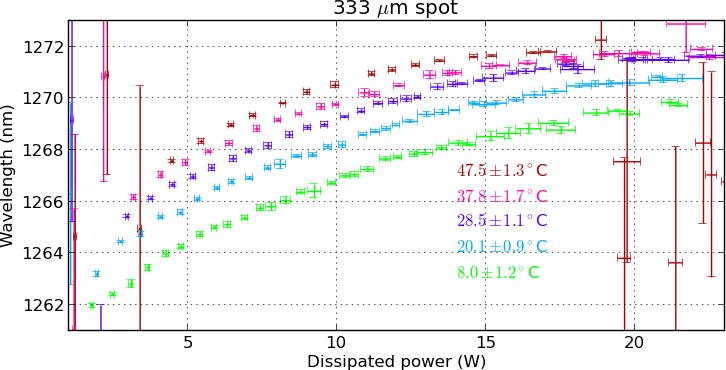
\includegraphics[width=14.5cm]{img/lambda_sample.png}
\caption{Longest emitted wavelength
recorded in the achromatic lens configuration
of sample 1.
The observed non-linear relation was not expected
given the discussion in section~\ref{sec:rth:lambda}.
The longest emitted wavelength
over all
seem to converge to a heat sink independent value.
This is in line with
the hypothesis of an intrinsic roll over temperature
suggested in section~\ref{sec:rth:trollover}.}
\label{img:lambda_sample}
\end{figure}

\begin{figure}
\centering
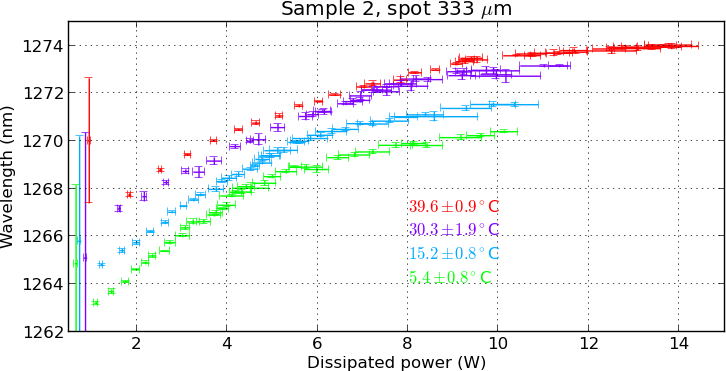
\includegraphics[width=14.5cm]{img/lambda_sampled6.png}
\caption{Longest emitted wavelength
recorded in the achromatic lens configuration
of sample 2.
The over all longest emitted wavelengths
appear not to converge
to the same value
for each of the heat sink temperatures.}
\label{img:lambda_sampled6}
\end{figure}